\chapter{Arquitectura y desarrollo}
\label{ch:arquitecturaydesarrollo}
\section{Solución propuesta}

Este proyecto propone una \gls{dapp} que gestiona préstamos de \gls{eth} dentro 
de la red \gls{ethereum} a través de \gls{smartcontract} desplegados en dicha
red.

Como se ha explicado en la comparación con otros protocolos \gls{defi}, 
la diferenciación de este sistema es que solo una entidad, poseedora del proyecto,
está autorizada a ofrecer los préstamos, configurar los tipos de préstamos
disponibles y gestionar los fondos.

El sistema se basa en \glspl{smartcontract} que registran en la red la
información necesaria para gestionar los préstamos. Estos contratos permiten
automatizar parte de la gestión y conservar un historial de las operaciones.

El usuario de la \gls{dapp} interactúa con el sistema a través de una interfaz web
en la que conectando su cartera con \gls{metamask} puede gestionar sus propios 
préstamos sin la necesidad de interactuar directamente con la organización del 
sistema.

El seguimiento de control de pagos de los contratos 
funciona como una máquina de estados automatizada que es accionada como un 
semáforo con ciclos mensuales.

En la figura~\ref{fig:semaforos} se pueden ver los tres tipos de estados en los que
puede encontrarse un préstamo al chequeo mensual de pagos (estado 0), cómo actúa la
\gls{dapp} dependiendo de su estado durante el chequeo (estado 1), y cómo queda
el préstamo pasado el chequeo esperando al próximo (estado 0).

\begin{figure}[H]
    \centering
    \caption{Diagrama de estados que asegura el control de
    los contratos del sistema.}
    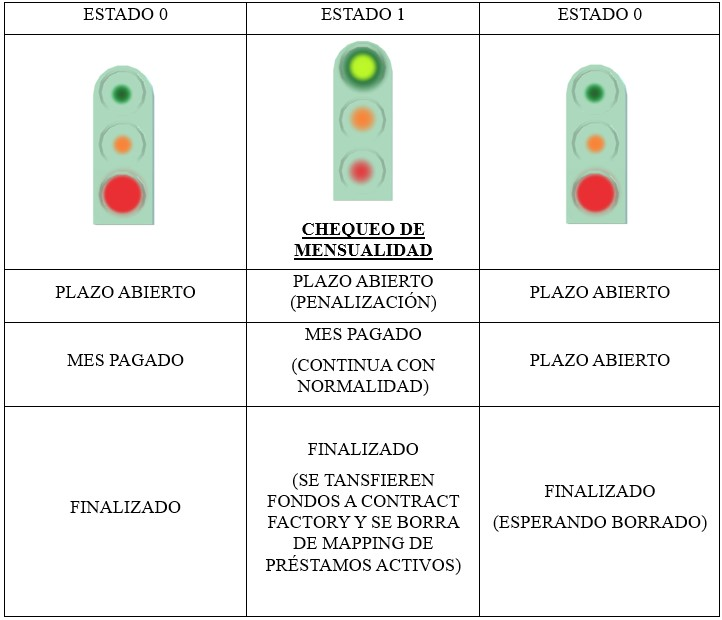
\includegraphics[width=\textwidth]{figures/semaforos.jpg}
    \label{fig:semaforos}
\end{figure}



\section{Limitaciones del proyecto}
\subsection{Limitaciones legales}
\label{subsec:limitaciones-legales}

Durante este proceso de desarrollo, en diciembre de 2024, la Unión Europea aprueba 
el Reglamento Europeo de Criptoactivos~\cite{[24]}. 
El objetivo de este reglamento es establecer normas para las entidades emisoras
y proveedoras de servicios relacionados con la criptoactividad.

En el nuevo reglamento se  tratan distintas cuestiones entre las que se 
encuentran:
\begin{enumerate}
    \item Requisitos de transparencia absoluta a las plataformas de negociación 
    de criptoactivos.
    \item Necesidad de autorización europea para la emisión y provisionamiento
    de criptoactivos.
    \item Protección del valor monetario en euros de los clientes.
    \item Creación de medidas de control de las operaciones con información 
    privilegiada y manipulación de mercado.
\end{enumerate}

En esta normativa se especifican acciones obligatorias para entidades financieras 
que pueden adoptar este proyecto. Dentro de estas acciones se definen elementos 
comunes a cualquier empresa como definirse como persona jurídica o actuar de forma 
honesta, justa y profesional.

Una de las exigencias que pueden limitar el proyecto es la obligatoriedad de ofrecer
la capacidad de convertir en euros los criptoactivos proporcionados por este
proyecto. Específicamente se obliga a mantener:
\begin{enumerate}
    \item Un fondo propio de 350\,000~\texteuro{}
    \item El 2\% del importe medio de los activos de reserva
    \item Una cuarta parte de los gastos generales fijos del año anterior
    \item Establecimiento de planes de recuperación y reembolso en caso de no 
    cumplir las obligaciones de la normativa 
\end{enumerate}

Estas acciones obligan a cualquier entidad que quiera hacer uso de este proyecto 
a aprovisionar las cantidades definidas en la normativa.

\subsection{Limitaciones técnicas}

El sistema desarrollado presenta una serie de limitaciones técnicas derivadas 
tanto del alcance definido para el proyecto como de las características propias de 
una solución basada en \glspl{smartcontract}. Las principales
limitaciones identificadas son las siguientes:

\begin{enumerate}
    \item \textbf{Pagos anticipados:} el sistema no contempla actualmente la
    realización de pagos anticipados sobre los préstamos contratados.

    \item \textbf{Cancelación anticipada:} no se contempla la posibilidad de
    cancelar un préstamo antes de que finalice el periodo establecido inicialmente
    en el momento de su contratación.

    \item \textbf{Ausencia de garantías o colateral:} el sistema no incorpora
    mecanismos de colateralización que permitan garantizar el pago del préstamo
    en caso de impago.

    \item \textbf{Uso de un único activo:} el prototipo utiliza exclusivamente
    \gls{eth} como activo para la concesión y devolución de los préstamos.
    No se contempla actualmente el uso de otros tokens o activos digitales como
    unidad de préstamo.

    \item \textbf{Escalabilidad y consumo de \gls{gas}:} el incremento del
    número de préstamos activos implica un mayor número de operaciones que deben
    ser procesadas y registradas en la \gls{blockchain}. En consecuencia, el coste
    acumulado de \gls{gas} puede aumentar a medida que crece el volumen de
    préstamos gestionados. Esta situación no tiene por qué invalidar el proyecto, pero sí exige un desarrollo orientado a mejorar su escalabilidad.
    \end{enumerate}

Estas limitaciones deben tenerse en cuenta al valorar una posible aplicación del
sistema en un entorno real a la vez que se plantean como líneas de desarrollo 
futuro.

\section{Análisis y diseño del software}
En esta sección se muestran diagramas y tablas que definen la estructura y 
el flujo del sistema.

\subsection{Actores del sistema}
Los actores que pueden participar en el sistema son:

\begin{itemize}
    \item \textbf{Usuario prestatario (User):} Usuario que accede al servicio de
    préstamos.
    \item \textbf{Entidad prestamista (Owner):} Entidad que ofrece los distintos
    tipos de préstamos.
\end{itemize}

\subsubsection{Diagrama UML}
En la figura~\ref{fig:uml} hay representado un \gls{diagramauml}
que relaciona los actores del sistema con los 
\enquote{Casos de Uso} que pueden realizar.

\begin{figure}[H]
    \centering
    \caption{Diagrama UML representando los actores del sistema relacionados 
    con los casos de uso a los que tienen acceso.}
    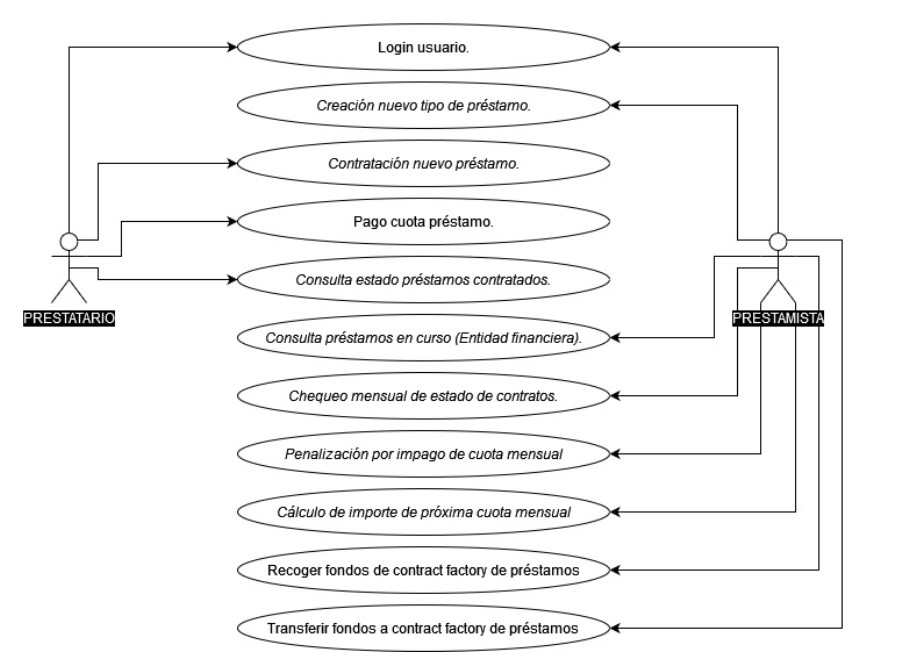
\includegraphics[width=\textwidth]{figures/uml.jpg}
    \label{fig:uml}
\end{figure}

\subsubsection{Diagrama de secuencia UML}
Para mostrar cómo interactúan los actores con el sistema en una línea de tiempo
y conocer el flujo de información que sucede en el sistema se ha definido
el siguiente \gls{secuenciauml} en la figura~\ref{fig:secuenciauml}.

En este caso, el diagrama de secuencia muestra cómo todo registro en el sistema
siempre es grabado en la \gls{blockchain}, siendo un flujo clave en este proyecto 
para poder dar las propiedades de veracidad e inmutabilidad a la información de los
préstamos.

\begin{figure}[H]
    \centering
    \caption{Diagrama de secuencia que representa cómo la información
    vital del sistema queda registrada en la red aportando las características 
    de inmutabilidad y confianza propias del proyecto.}
    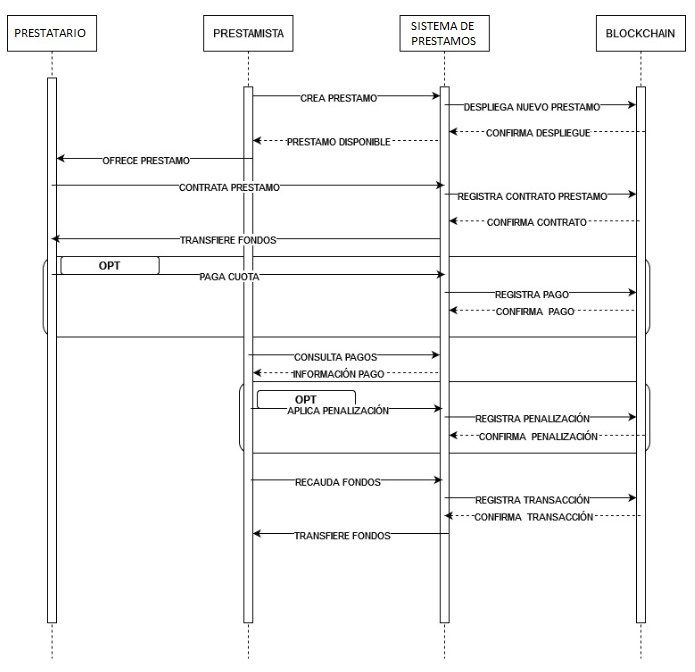
\includegraphics[width=\textwidth]{figures/diagramasecuencia.jpg}
    \label{fig:secuenciauml}
\end{figure}

\subsection{Casos de uso}

En el marco del desarrollo del presente proyecto, 
se ha priorizado la definición de un conjunto de casos de uso que representan 
los escenarios esenciales para cumplir con los objetivos fundamentales del 
sistema, de acuerdo con el alcance limitado del proyecto.

La selección de los casos de uso  no pretende abarcar una totalidad 
de posibles funcionalidades del sistema sino un conjunto operativo sólido y 
funcional, comentando también un posible desarrollo futuro.

Estos casos de uso se definen en las tablas ~\ref{tab:casos-uso-sistema} y 
~\ref{tab:casos-uso-posteriores}.

\subsubsection{Pantallas del sistema}
Para facilitar la comprensión de los casos de uso, se enumeran las principales
pantallas del sistema:

\begin{itemize}
    \item \textbf{Pantalla principal común:} Pantalla de inicio común a todos los
    usuarios, principalmente para identificarse en el sistema.
    \item \textbf{Pantalla principal del prestamista.}
    \item \textbf{Pantalla principal del prestatario.}
\end{itemize}

\subsubsection{Casos de uso}
\begin{table}[H]
\centering
\caption{Casos de uso del sistema}
\label{tab:casos-uso-sistema}
\small
\begin{tabular}{|c|l|c|c|}
    \hline
    \rowcolor[HTML]{D0E7FF}
    Código  & Descripción   & Prioridad & Dependencia  \\ \hline
    CU1     & Inicio de sesión usuario        & 10   &   \\ \hline
    CU2     & Creación nuevo tipo de préstamo     & 9   &   \\ \hline
    CU3     & Contratación nuevo préstamo        & 8   &  CU2 \\ \hline
    CU4     & Consulta estado préstamos contratados        & 7   & CU3   \\ \hline
    CU5     & Pago cuota préstamo       & 6   & CU3 \\ \hline
    CU6     & Consulta préstamos en curso (Entidad prestamista)        & 5   & CU3 \\ \hline
    CU7     & Chequeo mensual de estado de contratos        & 4   &   \\ \hline
    CU8     & Penalización por impago de cuota mensual       & 3   &CU7   \\ \hline
    CU9     & Cálculo de importe de próxima cuota mensual         & 2   &  CU3  \\ \hline
    CU10     & Retirar fondos del sistema        & 1   &   \\ \hline
    CU11     & Ingresar fondos en el sistema        & 1   &   \\ \hline
\end{tabular}
\end{table}


\subsubsection{Casos de uso para posteriores desarrollos}


    \begin{table}[H]
    \centering
    \caption{Casos de uso para desarrollos posteriores}
    \label{tab:casos-uso-posteriores}
    \begin{tabular}{|c|l|}
        \hline
        \rowcolor[HTML]{D0E7FF}
    Código & Descripción \\ \hline
    \hypertarget{cu:garantia}{CU12}
        & Garantía de devolución en caso de impago \\ \hline
    \hypertarget{cu:euribor}{CU13}
        & Consulta del valor del \gls{euribor} \\ \hline
    \hypertarget{cu:solvencia}{CU14}
        & Validación de solvencia económica de usuarios \\ \hline
    \end{tabular}
    \end{table}

\subsubsection{Casos de uso detallados}
En esta sección se describen los casos de uso implementados y más adelante,
en la sección de trabajo futuro se comentarán los casos de uso futuros.

\begin{table}[H]
\centering
\caption{Casos de uso 1}
\begin{tabular}{|c|p{12cm}|}
    \hline
    \rowcolor[HTML]{D0E7FF}
    CU1 & \gls{login} del usuario. \\ \hline
    Descripción   & Los usuarios se identificarán en el sistema a través de MetaMask.  \\ \hline
    Pantalla     & Pantalla inicial. (Se redirecciona a esta página si no se ha realizado el \gls{login}).   \\ \hline
    Rol     & Cualquier usuario. \\ \hline
    Flujo     &    - El usuario, al acceder a la página web, recibirá una notificación
    por parte de MetaMask  para poder acceder al
                           servicio. \newline
                   - La extensión de MetaMask permite la autenticación del          usuario y la página se redirige a la página correspondiente a su rol.
    \\ \hline
\end{tabular}
\end{table}

\begin{table}[H]
\centering
\caption{Casos de uso 2}
\begin{tabular}{|c|p{12cm}|}
    \hline
    \rowcolor[HTML]{D0E7FF}
    CU2 & Creación nuevo tipo de préstamo. \\ \hline
    Descripción   & La entidad prestamista puede crear nuevos productos tipo \enquote{préstamo}.  \\ \hline
    Pantalla     & Pantalla principal de la entidad prestamista.  \\ \hline
    Rol     & Owner. \\ \hline
    Flujo     &    - El usuario owner tiene un formulario en su página principal para
rellenar la información necesaria para la creación de un nuevo tipo de
préstamo.\newline
                   - Este contrato se le mostrará al usuario prestatario en su página principal en forma de producto para contratar.
                 \\ \hline
\end{tabular}
\end{table}

\begin{table}[H]
\centering
\caption{Casos de uso 3}
\begin{tabular}{|c|p{12cm}|}
    \hline
    \rowcolor[HTML]{D0E7FF}
    CU3 & Contratación nuevo préstamo. \\ \hline
    Descripción   & Los usuarios prestatarios pueden seleccionar el préstamo que desean contratar.  \\ \hline
    Pantalla     & Pantalla principal de usuarios prestatarios.   \\ \hline
    Rol     & User. \\ \hline
    Flujo     &    - En la página principal el usuario podrá visualizar los posibles préstamos que
puede contratar. \newline
                   - El usuario contrata un nuevo préstamo pinchando en el botón de
\enquote{Contratar}. \newline
                                 Tan pronto como se procese la transacción, la \gls{dapp} llamará al \gls{smartcontract} desplegado en la red el cual genera otro \gls{smartcontract} que refleja el estado del préstamo en
cada momento. \newline
                                Al mismo tiempo, las unidades de \gls{eth} solicitadas en el préstamo serán transferidas
automáticamente desde los fondos del \gls{smartcontract} que conserva el balance del sistema a la dirección del
usuario.
                  \\ \hline
\end{tabular}
\end{table}

\begin{table}[H]
\centering
\caption{Casos de uso 4}
\begin{tabular}{|c|p{12cm}|}
    \hline
    \rowcolor[HTML]{D0E7FF}
    CU4 & Consulta estado préstamos contratados. \\ \hline
    Descripción   & Los usuarios del servicio podrán consultar el estado de sus préstamos contratados
visualizándolos en su página principal.  \\ \hline
    Pantalla     & Pantalla principal usuario.   \\ \hline
    Rol     & User. \\ \hline
    Flujo     &    En el momento en que el usuario hace inicio de sesión ya puede visualizar los contratos
que tiene contratados. \\ \hline
                 
\end{tabular}
\end{table}

\begin{table}[H]
    \centering
    \caption{Casos de uso 5}
\begin{tabular}{|c|p{12cm}|}
    \hline
    \rowcolor[HTML]{D0E7FF}
    CU5 & Pago cuota préstamo. \\ \hline
    Descripción   & Los usuarios del servicio de préstamo realizan el pago de sus 
    mensualidades a través de la \gls{dapp} del proyecto.  \\ \hline
    Pantalla     & Pantalla principal de usuarios prestatarios.   \\ \hline
    Rol     & User. \\ \hline
    Flujo     &    - En la página principal del usuario aparecen los distintos préstamos que
tiene contratados y sus respectivos estados, junto a esto, existe un botón para
cada contrato que transfiere la mensualidad calculada previamente desde la
cuenta del usuario a la dirección del \gls{smartcontract} de préstamo.
                 \\ \hline
\end{tabular}
\end{table}

\begin{table}[H]
\centering
\caption{Casos de uso 6}
\begin{tabular}{|c|p{12cm}|}
    \hline
    \rowcolor[HTML]{D0E7FF}
    CU6 & Consulta préstamos en curso (Entidad prestamista). \\ \hline
    Descripción   & La entidad prestamista puede consultar el estado de cada préstamo en
curso. \\ \hline
    Pantalla     &Pantalla principal de la entidad prestamista.  \\ \hline
    Rol     & Owner. \\ \hline
    Flujo     &    - En la página principal del propietario aparecen los contratos en curso.
                 \\ \hline
\end{tabular}
\end{table}

\begin{table}[H]
\centering
\caption{Casos de uso 7}
\begin{tabular}{|c|p{12cm}|}
    \hline
    \rowcolor[HTML]{D0E7FF}
    CU7 & Chequeo mensual de estado de contratos. \\ \hline
    Descripción   & La entidad prestamista ejecuta la orden de comprobar qué mensualidades no
han sido pagadas ese mes.  \\ \hline
    Pantalla     & Pantalla principal de entidad prestamista. \\ \hline
    Rol     & Owner. \\ \hline
    Flujo     &    Desde la página principal del propietario se tiene acceso al botón que lanza
esa orden siempre y cuando hayan pasado 30 días desde la última orden.
                 \\ \hline
\end{tabular}
\end{table}

\begin{table}[H]
\centering
\caption{Casos de uso 8}
\begin{tabular}{|c|p{12cm}|}
    \hline
    \rowcolor[HTML]{D0E7FF}
    CU8 & Penalización por impago de cuota mensual. \\ \hline
    Descripción   & Los contratos en estado de impago generan una penalización de deuda, esta
penalización solo puede suceder una vez al mes.  \\ \hline
    Pantalla     & Pantalla principal de entidad prestamista.  \\ \hline
    Rol     & Owner. \\ \hline
    Flujo     &    Cuando el propietario genera la orden de chequeo mensual los contratos
que tengan estado de \enquote{impago} aumentarán su valor de deuda.
                 \\ \hline
\end{tabular}
\end{table}

\begin{table}[H]
\centering
\caption{Casos de uso 9}
\begin{tabular}{|c|p{12cm}|}
    \hline
    \rowcolor[HTML]{D0E7FF}
    CU9 & Cálculo de importe de próxima cuota mensual. \\ \hline
    Descripción   & El importe de la próxima cuota mensual es un valor dinámico sujeto a
penalizaciones.  \\ \hline
    Pantalla     & Pantalla principal usuario.  \\ \hline
    Rol     & User. \\ \hline
    Flujo     &    - Tras el chequeo mensual la cuota del próximo pago se podrá ver
modificada en caso de penalización. \newline
                   - En la información de los préstamos contratados aparecerá la cantidad de la
cuota del mes en curso.
                 \\ \hline
\end{tabular}
\end{table}

\begin{table}[H]
\centering
\caption{Casos de uso 10}
\begin{tabular}{|c|p{12cm}|}
    \hline
    \rowcolor[HTML]{D0E7FF}
    CU10 & Retirar fondos del sistema. \\ \hline
    Descripción   & La entidad prestamista propietaria  del sistema de préstamos puede disponer de los fondos almacenados en el sistema
cuando desee.  \\ \hline
    Pantalla     & Pantalla principal de Owner.   \\ \hline
    Rol     & Owner. \\ \hline
    Flujo     &    La entidad prestamista tendrá una casilla en su página principal para escribir y recibir el
importe desde la dirección del \gls{smartcontract} con el balance a su dirección de la red.
                 \\ \hline
\end{tabular}
\end{table}

\begin{table}[H]
\centering
\caption{Casos de uso 11}
\begin{tabular}{|c|p{12cm}|}
    \hline
    \rowcolor[HTML]{D0E7FF}
    CU11 & Ingresar fondos en el sistema. \\ \hline
    Descripción   & La entidad prestamista  puede transferir cualquier cantidad de \gls{eth}
    al sistema de préstamos para mantener
 un saldo positivo y poder realizar estos préstamos.\\ \hline
    Pantalla     & Pantalla principal Owner.   \\ \hline
    Rol     & Owner. \\ \hline
    Flujo     &    La entidad tendrá una casilla en su página principal para escribir y transferir el
importe deseado a la dirección del sistema de préstamos.
                 \\ \hline
\end{tabular}
\end{table}

\clearpage
\subsection{Entidades del sistema}
A continuación se definen las entidades cuyas relaciones compondrán y 
habilitarán las funciones del sistema propuesto.

\begin{table}[H]
\centering
\caption{Definición de entidades del sistema}
\begin{tabular}{|c|p{12cm}|}
    \hline
    \rowcolor[HTML]{D0E7FF}
    1 & Usuario. \\ \hline
    Descripción   & Usuario que accede al servicio de préstamos.  \\ \hline
    Atributos     & Dirección pública de la red.   \\ \hline
    Acciones     &- Pedir préstamo.  \newline
                    - Pagar préstamo.\\ \hline

    \hline
    \rowcolor[HTML]{D0E7FF}
    2 & Propietario. \\ \hline
    Descripción   & Propietario del sistema, único capaz de recolectar los fondos del sistema. Normalmente una entidad prestamista.  \\ \hline
    Atributos     & Dirección pública de la red.   \\ \hline
    Acciones     &- Transferir unidades al sistema. \newline
                    - Recoger unidades del sistema.\\ \hline
   

    \hline
    \rowcolor[HTML]{D0E7FF}
    3 & Sistema de préstamos.     \\ \hline
    Descripción   & Conjunto de \glspl{smartcontract} que definen los elementos del sistema y cuya ejecución valida las transacciones del sistema.  \\ \hline
    Atributos     &- Dirección de propietario. \newline
                    - Lista de préstamos contratables. \newline
                    - Lista de usuarios junto con sus préstamos en curso.\\ \hline
    Acciones     & - Ejecutar las transacciones ordenadas por los usuarios del sistema.  \newline
                    - Registrar en la red \gls{ethereum} la información del sistema.\\ \hline
   
\end{tabular}
\end{table}

\clearpage
\subsubsection{Diagrama de entidad-relación}
El  diagrama  representado en la figura~\ref{fig:er} pretende 
definir mediante relaciones entre las entidades las funciones que 
definen el sistema.
\begin{figure}[H]
    \centering
    \caption{Diagrama de entidad-relación.}
    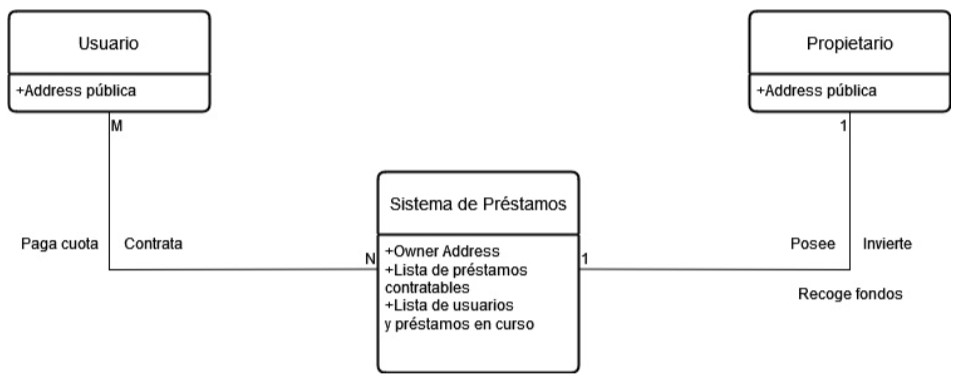
\includegraphics[width=\textwidth]{figures/E-R.jpg}
    \label{fig:er}
\end{figure}

\section{Análisis de los contratos inteligentes implicados}

En esta sección se define la arquitectura de diseño utilizada para los 
\glspl{smartcontract}, así como los atributos (tablas~\ref{fig:atributosfactory} y \ref{fig:atributosprestamo}) y 
funciones (tablas~\ref{fig:funcionesfactory} y \ref{fig:funcionesprestamo}) de 
cada uno de ellos.

\subsection{Diagrama de entidad-relación de contratos inteligentes}

Aunque no sean entidades del sistema, para explicar detalladamente la arquitectura 
de diseño se define otro diagrama de entidad-relación en la
figura~\ref{fig:ersmartcontract}.

\begin{figure}[H]
    \centering
    \caption{Diagrama de entidad-relación que representa las relaciones y funciones entre los contratos inteligentes.}
    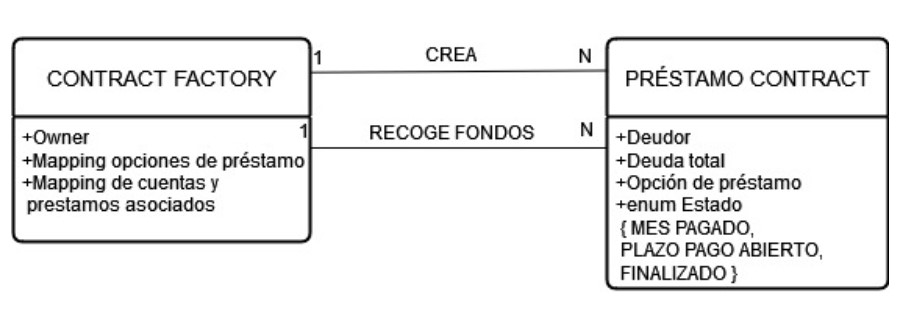
\includegraphics[width=\textwidth]{figures/E-R-smartcontracts.jpg}
    \label{fig:ersmartcontract}
\end{figure}
\subsubsection{PrestamosFactory}
La figura~\ref{fig:ersmartcontract} también define gráficamente el
patrón de diseño utilizado en el desarrollo de los \glspl{smartcontract}. A este
patrón se le denomina \enquote{Factory}.

El diseño de \enquote{Factory} encaja perfectamente en el desarrollo
de este proyecto ya 
que nos permite crear los distintos contratos de préstamo
de forma dinámica y automática.
En esta arquitectura, un contrato principal (el \textit{Factory}) actúa como 
intermediario recibiendo las solicitudes y generando nuevos contratos 
(\textit{contratos préstamo}) según
las necesidades de los usuarios o la aplicación.
Dentro de este contrato se definen los distintos tipos de préstamos que pueden 
ser contratados por los usuarios,
así como las distintas funcionalidades de gestión y monitorización.
Para ello este contrato cuenta con variables como las del fragmento de código siguiente:
\begin{lstlisting}[language=Solidity, caption={Registro de préstamos en curso por usuario},label={lst:prestamoscursando}]
    mapping(address => PrestamoCursando[])  prestamosCursando;
    address[] clientes;
\end{lstlisting}
En el fragmento de código del listado~\ref{lst:prestamoscursando} se observa 
la variable \textit{prestamosCursando} perteneciente al \gls{smartcontract} principal
\textit{PrestamosFactory}, la cual guarda en la red \gls{blockchain} el
conjunto de direcciones correspondientes a un contrato tipo \textit{Préstamo} 
pertenecientes al sistema.

Por otra parte, cada contrato creado por \textit{PrestamosFactory}, es decir, cada contrato de préstamo, mantiene información específica como la dirección
del prestatario, la deuda restante, el número de cuotas pendientes, 
el estado del préstamo o el porcentaje de penalización aplicable, tal y como 
se muestra en el fragmento de código~\ref{lst:prestamovariables}.



        \begin{lstlisting}[language=Solidity, 
            caption={Variables contrato préstamo},
            label={lst:prestamovariables}]
            uint index;
            enum State { PAGADO, ABIERTO, FINALIZADO }
            State state;
            address prestatario;
            address entidadFinanciera;
            address payable prestamosFactory;
            uint256 cuotasRestantes;
            uint256 cantidadPrestada;
            uint256 deudaRestante;
            uint256 cuotaMensual;
            uint256 penalizacion;
            uint256 ultimoCheckeo;
        \end{lstlisting}



\subsection{Análisis de contratos inteligentes}
\subsubsection{PrestamosFactory }
El contrato \textit{PrestamosFactory} centraliza la gestión de los tipos de
préstamo disponibles y el registro de los préstamos asociados a cada usuario. 
Para ello, mantiene un conjunto de atributos que identifican al propietario del 
sistema, definen las condiciones de los productos y 
relacionan a los usuarios con sus contratos de préstamo. 
La tabla~\ref{fig:atributosfactory} recoge estos atributos.
    \begin{table}[H]
    \centering
    \caption{Descripción de atributos del Contrato PrestamosFactory}
        \label{fig:atributosfactory}
    \small
    \begin{tabular}{|p{3cm}|p{4.1cm}|p{6.1cm}|}
        \hline
        \rowcolor[HTML]{D0E7FF}
        Nombre & Tipo de dato & Descripción\\ \hline
        Owner&\gls{addresstype}&Dirección de la red \gls{ethereum} perteneciente a la 
        propietaria del sistema.\\ \hline
        Tipos de préstamo&\texttt{TipoContrato[]}&Array que guarda los tipos de préstamo contratables por el usuario. \newline
    Esta variable solo puede ser editada si el usuario se identifica con la dirección del propietario.\\ \hline
    TipoPréstamo&Struct&Conjunto de variables que definen un tipo de préstamo (importe, intereses, deuda total, penalización de impago y  cuotas)\\ \hline
    Préstamos en curso&\texttt{mapping(address =>}\newline\texttt{Prestamo\allowbreak{}Cursando[])}&Mapping que relaciona la dirección de un
    usuario con las direcciones de sus
    préstamos en curso. \newline
    El contrato principal actualiza este registro al contratar o eliminar un préstamo.\\ \hline
    \end{tabular}
    \end{table}


A continuación, la tabla~\ref{fig:funcionesfactory} presenta las funciones del contrato
\textit{PrestamosFactory}, sus parámetros de entrada y salida y una
descripción de su finalidad.

\begin{table}[H]
\centering
\caption{Descripción de funciones del Contrato PrestamosFactory}
\label{fig:funcionesfactory}
\small
\begin{tabular}{|p{3.5cm}|p{3cm}|p{2.1cm}|p{4.4cm}|}
\hline
\rowcolor[HTML]{D0E7FF}
Nombre & Entrada & Salida & Descripción \\ \hline
\texttt{definir\allowbreak{}Prestamo} & Interés, importe, cuotas y penalización & --- & Crea un tipo de préstamo y emite el evento correspondiente. Solo puede ejecutarla el propietario. \\ \hline
\texttt{contratar\allowbreak{}Prestamo} & Prestatario e índice del tipo & --- & Crea un contrato individual, lo registra y transfiere el importe al prestatario. \\ \hline
\texttt{get\allowbreak{}Clientes} & --- & Direcciones & Devuelve las direcciones de los clientes registrados. Solo puede consultarlas el propietario. \\ \hline
\texttt{recolectar\allowbreak{}Fondos} & Importe & --- & Transfiere fondos del contrato principal al propietario. \\ \hline
\texttt{invertir} & Valor de la transacción & --- & Recibe fondos en el contrato principal y emite un evento. \\ \hline
\texttt{ver\allowbreak{}Contratos} & Dirección del prestatario & Contratos de préstamo & Devuelve los contratos asociados al usuario. Solo pueden consultarlos el propietario o el prestatario. \\ \hline
\texttt{ver\allowbreak{}Tipos\allowbreak{}Contrato} & --- & Tipos de préstamo & Devuelve los productos disponibles. \\ \hline
\texttt{get\allowbreak{}Balance} & --- & Saldo & Devuelve el saldo del contrato principal al propietario. \\ \hline
\texttt{eliminar\allowbreak{}Prestamo\allowbreak{}Finalizado} & Usuario e índice & --- & Elimina del registro un préstamo finalizado y actualiza los índices. \\ \hline
\end{tabular}
\end{table}


\subsubsection{PrestamoCursando }

El \gls{smartcontract} \texttt{PrestamoCursando} representa un préstamo
individual contratado por un usuario. 
Almacena las condiciones del préstamo, permite el pago de las
cuotas y mantiene actualizado su estado tras el chequeo de mensualidad.
A continuación, en la tabla~\ref{fig:atributosprestamo} se describen
los atributos implicados.

\begin{table}[H]
\centering
\caption{Descripción de atributos del Contrato PrestamoCursando }
\label{fig:atributosprestamo}
\small
\begin{tabular}{|p{3.4cm}|p{2.5cm}|p{7cm}|}
\hline
\rowcolor[HTML]{D0E7FF}
Nombre & Tipo de dato & Descripción \\ \hline
\texttt{index} & \texttt{uint} & Posición del préstamo en el registro del usuario. \\ \hline
\texttt{state} & \texttt{State} & Estado: \texttt{PAGADO}, \texttt{ABIERTO} o \texttt{FINALIZADO}. \\ \hline
\texttt{cuotas\allowbreak{}Restantes} & \texttt{uint256} & Número de mensualidades pendientes. \\ \hline
\texttt{prestatario} & \texttt{address} & Dirección de la cuenta que contrata el préstamo. \\ \hline
\texttt{deudaRestante} & \texttt{uint256} & Deuda pendiente, expresada en wei. \\ \hline
\texttt{cuotaMensual} & \texttt{uint256} & Importe de la próxima cuota, expresado en wei. \\ \hline
\texttt{penalizacion} & \texttt{uint256} & Porcentaje aplicado a la deuda en caso de impago. \\ \hline
\end{tabular}
\end{table}

El encargado de las operaciones de actualización de importes del \textit{contrato de préstamo}
es el propio \gls{smartcontract} a través de las funciones explicadas en la tabla~\ref{fig:funcionesprestamo}.

\begin{table}[H]
\centering
\caption{Descripción de funciones del Contrato PrestamoCursando }
    \label{fig:funcionesprestamo}
\small
\begin{tabular}{|p{4.2cm}|p{2cm}|p{2cm}|p{4.8cm}|}
\hline
\rowcolor[HTML]{D0E7FF}
Nombre & Entrada & Salida & Descripción \\ \hline
\texttt{pagarMensualidad} & Valor de la cuota & --- & Comprueba el pago, actualiza deuda y estado y envía los fondos al contrato principal. \\ \hline
\texttt{penalizarPrestamo} & --- & --- & Función privada que aumenta la deuda por impago y recalcula la cuota. \\ \hline
\texttt{calculo\allowbreak{}Cuota\allowbreak{}Mensual} & --- & Cuota en wei & Función privada que calcula la cuota; incorpora el resto de la división a la última mensualidad. \\ \hline
\texttt{checkeoMensual} & --- & --- & Actualiza el estado y aplica la penalización o elimina el préstamo finalizado. Exige el plazo y la cuenta de la entidad prestamista. \\ \hline
\end{tabular}
\end{table}

\subsection{Decisiones de implementación en el sistema}

Durante el desarrollo de los \glspl{smartcontract} se han tomado decisiones
técnicas sobre la distribución de responsabilidades entre la aplicación y la red,
el control de acceso y el registro de las transacciones. A continuación, se
presentan las principales decisiones adoptadas.

\paragraph{Controles de acceso reflejados en la propia red:}
Al contar cada \textit{contrato de préstamo} con su propia información,
se garantiza que 
cada préstamo es independiente y el sistema de control de acceso puede 
ser gestionado de manera casi autónoma si está reflejado en la \gls{blockchain}. 

Se puede ver un ejemplo de gestión autónoma en la función del fragmento de código~\ref{lst:funcionpagarmensualidad}
 del 
\textit{contrato de préstamo}, en la que a través de las líneas que comienzan por
\lstinline[language=Solidity]|require|, aseguramos que:
\begin{itemize}
    \item El 
prestatario sea el único que puede realizar el pago de la mensualidad.
\item El importe enviado es exactamente el valor de la cuota mensual
\item El estado del préstamo permite realizar el pago.
\end{itemize} 

        \begin{lstlisting}[language=Solidity, caption={Función para pagar mensualidad},label={lst:funcionpagarmensualidad}]
            function pagarMensualidad() payable public {
                require(msg.sender == prestatario, "Only borrower");
                require(msg.value == cuotaMensual, "Send exact debt value");
                require(state == State.ABIERTO, "Payment period not open");
            
                state = State.PAGADO;
                deudaRestante -= cuotaMensual;
                cuotasRestantes--;

                if(cuotasRestantes == 1){   cuotaMensual = calculoCuotaMensual(); }

                if(cuotasRestantes == 0){  state = State.FINALIZADO;  }
                transferirFondosAFactory(msg.value);  }
        \end{lstlisting}



\paragraph{Contrato préstamo \textit{abstracto}}
Para que la creación de varios tipos de \textit{contrato de préstamo}  sea dinámica
y se puedan definir desde la \gls{dapp} 
se ha optado por crear un único contrato que pueda ser parametrizado en el 
momento de su creación.
En el contrato \textit{factory} se define una estructura, mostrada en el fragmento de código~\ref{lst:structtipocontrato}, que contiene los
parámetros de cada tipo de préstamo, como el importe, los intereses, 
la penalización por impago y el número de cuotas. 
            \begin{lstlisting}[language=Solidity, caption={struct TipoContrato},label={lst:structtipocontrato}] 
                struct TipoContrato {
                    uint256 index;
                    uint256 porcentajeInteres; 
                    uint256 cantidad; 
                    uint256 deudaTotal;
                    uint256 cuotas;
                    uint256 penalizacionImpago;
                }
            \end{lstlisting}
            
Cuando un usuario solicita un préstamo, 
se pasa el tipo de préstamo seleccionado al constructor del contrato de préstamo, mostrado en el fragmento de código~\ref{lst:constructorprestamo},
que inicializa sus variables con los valores correspondientes.
            \begin{lstlisting}[language=Solidity, caption={Constructor de PrestamoCursando},label={lst:constructorprestamo}]
                constructor(uint256 _index, address _prestatario, address _entidad, uint256 _cuotasRestantes, uint256 _cantidad, uint256 _deudaTotal, uint256 _penalizacion){
                    index = _index;
                    state = State.ABIERTO;
                    prestatario = _prestatario;
                    entidadFinanciera = _entidad;
                    prestamosFactory = payable(msg.sender);
                    cuotasRestantes = _cuotasRestantes;
                    cantidadPrestada = _cantidad;
                    deudaRestante = _deudaTotal;
                    penalizacion = _penalizacion;
                    cuotaMensual = calculoCuotaMensual();
                    ultimoCheckeo = block.timestamp;
                }
            \end{lstlisting}
\subsubsection{Direcciones como identificación}
En un sistema basado en \gls{ethereum} no es necesario generar un identificador centralizado para identificar a un usuario.
La dirección pública de su cartera constituye un identificador único dentro de la red.
Cada solicitud de préstamo genera un nuevo contrato con una dirección propia.
El contrato principal registra su asociación con el prestatario en la variable
\texttt{prestamosCursando}. De este modo, se pueden consultar y administrar los
préstamos vinculados a cada usuario mediante la función del
fragmento de código~\ref{lst:funcionvercontratos}.

\begin{lstlisting}[language=Solidity, caption={Función que devuelve los contratos de un usuario},label={lst:funcionvercontratos}]
     function verContratos(address _prestatario) public view returns (PrestamoCursando[] memory){
        require((msg.sender == owner)||(msg.sender == _prestatario), "Top Secret");
        return (prestamosCursando[_prestatario]);
    }
\end{lstlisting}

\subsubsection{Representación de cantidades monetarias} 
Las cantidades monetarias se almacenan como enteros sin signo de tipo
\texttt{uint256}, expresados en \gls{wei}. La división entre enteros en Solidity
trunca el resultado hacia cero~\cite{solidityTipos}. Por ello, el cálculo de una
cuota puede dejar un resto; el contrato incorpora ese resto a la última cuota.


\subsubsection{Reducción del consumo de gas} 
Siempre que una operación no requiere necesariamente modificar el estado de 
la blockchain, esta se ejecuta en la aplicación web del cliente. 
De esta manera se evita utilizar \gls{gas} para operaciones puramente 
relacionadas con la visualización de información, como el recorrido de los 
contratos de un usuario para mostrar su estado. 
En este sistema se recupera la información de todos los contratos~\ref{lst:recuperacioncontratos} 
 y es la 
aplicación web la que filtra y muestra la información de cada contrato (fragmento de código~\ref{lst:funcionvercontratosweb}). El primer fragmento de código recupera la información de la red
y el segundo la muestra por pantalla al usuario.

    \begin{lstlisting}[language=TypeScript, caption={Recuperación de información de contratos},label={lst:recuperacioncontratos}]
        async iniciarVistaContratados(){
    this.direccionesContratados = await this.factoryContract.methods
        .verContratos(localStorage.getItem('userAddress'))
            .call({ from: localStorage.getItem('userAddress')});

        this.direccionesContratados.forEach(async (direccion: any) => {
        var prestamoCursando = new this.web3.eth.Contract(PRESTAMOCURSANDO.abi, direccion);
        var contratado = await prestamoCursando.methods.mostrarInfo().call({from: localStorage.getItem('userAddress')});
        contratado._ultimoCheckeo = this.secondsToDateString(contratado._ultimoCheckeo);
        contratado._state = this.contratoStateToString(contratado._state);
        this.listaContratados.push(contratado);
        });
  }
\end{lstlisting}
    \begin{lstlisting}[language=HTML, caption={Muestra de información de contratos},label={lst:funcionvercontratosweb}]
<ion-col *ngFor="let prestamo of listaContratados;" size="3.1"  >
      <ion-card >
        <ion-card-content >
          <ion-list >
            <ion-item > <ion-label  class = "ion-text-center" >Estado: {{ prestamo._state.toString() }}</ion-label> </ion-item>
            <ion-item > <ion-label  class = "ion-text-center" >Deuda Restante: {{ prestamo._deudaRestante.toString() }}</ion-label> </ion-item>
            <ion-item > <ion-label class = "ion-text-center" >Cuotas Restantes: {{ prestamo._cuotasRestantes.toString() }} </ion-label> </ion-item>
            <ion-item > <ion-label class = "ion-text-center" >Cantidad Próxima Cuota: {{ prestamo._cuotaMensual.toString() }} </ion-label> </ion-item>
            <ion-item > <ion-label class = "ion-text-center">Fin del plazo actual: {{ prestamo._ultimoCheckeo }}</ion-label> </ion-item>
            <ion-item> <ion-label class = "ion-text-center">Penalización por Impago: {{ prestamo._penalizacionImpago.toString() }}%</ion-label> </ion-item>  
          </ion-list>
          <ion-button (click)="pagarCuota(prestamo._direccion, prestamo._cuotaMensual)">PAGAR CUOTA ({{prestamo._cuotaMensual.toString()}})</ion-button>
        </ion-card-content>
      </ion-card>
</ion-col>
\end{lstlisting}

\subsubsection{Registro del estado antes de realizar transferencias} 
En Solidity es una buena práctica validar las condiciones de una operación y
actualizar el estado del contrato antes de realizar transferencias de fondos.

Existe un tipo de ataque llamado \textit{Ataque por reentrada}.
En este ataque el riesgo se produce cuando un \gls{smartcontract} transfiere 
fondos a otro contrato y este aprovecha la ejecución de su código para volver a 
invocar una función del contrato original antes de que termine la operación 
inicial. Si todavía no se han actualizado las variables de saldos, el atacante
podría repetir una retirada utilizando un estado de las variables desactualizado y
llegar a extraer fondos indebidamente. 

Se puede ver cómo se realiza en este proyecto una transferencia de saldo en
el fragmento de código~\ref{lst:funcionpagarmensualidad}.


Para un mayor entendimiento de este tipo de ataques se añade la 
figura~\ref{fig:ataque-reentrada}
con un gráfico poniendo un ejemplo con una transferencia de 10 \gls{eth}.
\begin{figure}[H]
    \centering
    \caption{Diagrama de un ataque de reentrada}
    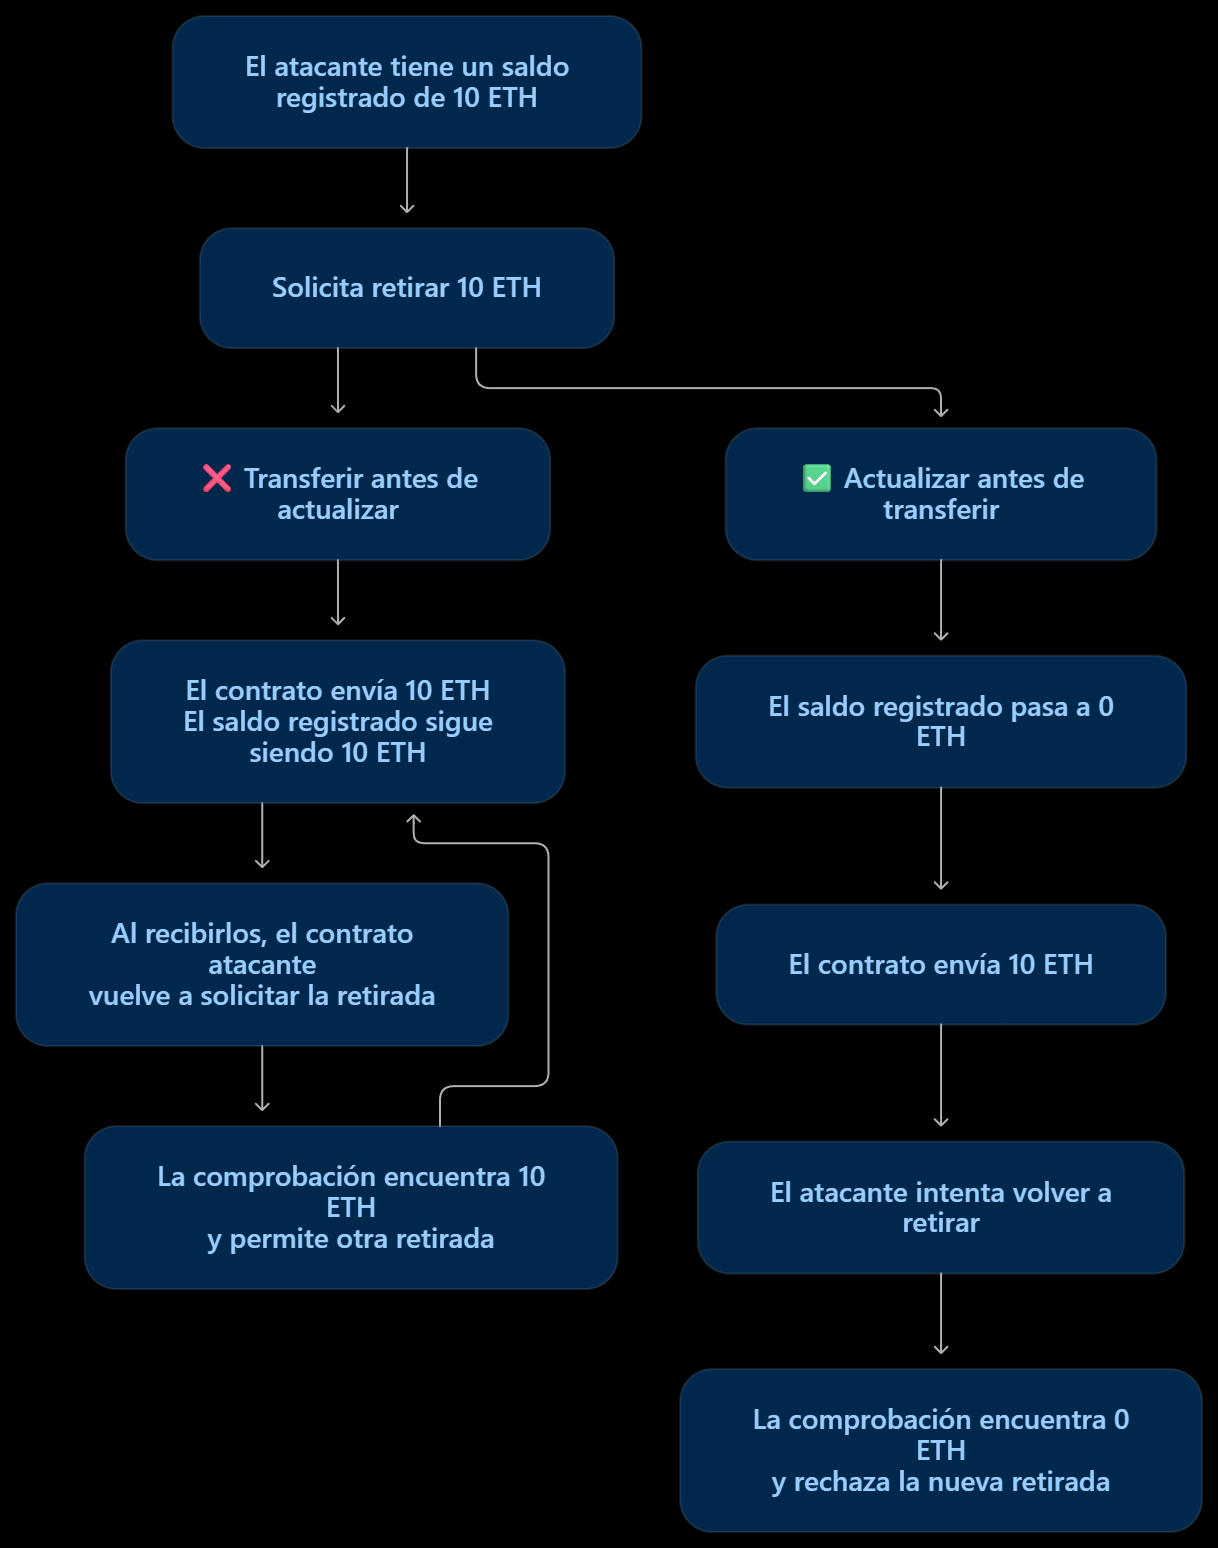
\includegraphics[width=\textwidth]{figures/ataqueReentrada-diagram.png}
    \label{fig:ataque-reentrada}
\end{figure}



\section{Validación de resultados}
\subsection{Validación a través del uso de la aplicación del sistema}
Tras el desarrollo del sistema de préstamos descentralizado, es necesario 
comprobar si cumple con los objetivos planteados y cubre los casos de uso 
definidos. 
Para ello, se ha realizado manualmente un flujo de uso de la interfaz de usuario y
se presentan pruebas mediante capturas de pantalla de la interfaz 
y registros en la herramienta \textit{Etherscan} para validar la ejecución de 
las transacciones y el correcto funcionamiento de los \glspl{smartcontract}
en la \gls{blockchain} de \gls{ethereum}.
Para comprender las siguientes imágenes es importante conocer 
los siguientes conceptos:

\begin{enumerate}
    \item \textbf{Wei:} En la red \gls{ethereum} es la unidad más pequeña de valor 
    para su criptomoneda \gls{eth}. Un \gls{eth} está compuesto por un total de 
    $10^{18}$ wei.
    \item Las cadenas de caracteres que comienzan por \texttt{'0x'} en la red 
    \gls{ethereum} están reservadas como direcciones que pueden apuntar a 
    usuarios, entidades o \glspl{smartcontract}.
    
\end{enumerate}


El \gls{op}~\ref{op:2} consiste en la unificación de las distintas funcionalidades 
del proyecto en una interfaz accesible a cualquier sujeto independientemente de su formación.
Los resultados se podrán ver a lo largo de la sección y se podrá apreciar que, aunque la 
interfaz sí reúne todas las funcionalidades del sistema, no se ha hecho hincapié en la
accesibilidad e intuitividad. 
Durante el desarrollo del proyecto se ha decidido aportar más esfuerzo en la funcionalidad 
dejando la evolución de la interfaz de usuario a un estado más \textit{amigable} para
trabajo futuro.

Para la validación de resultados del \gls{op}~\ref{op:1} se pueden evaluar los distintos objetivos secundarios:
\begin{enumerate}
    \item \textbf{\gls{os}~\ref{os:1}:} La aplicación solicita a \gls{metamask} la
    conexión de una cuenta y la autorización de las operaciones. La dirección
    permite asociar los préstamos a una cuenta. La figura~\ref{fig:metamask} muestra
    este acceso a la aplicación.

    \begin{figure}[H]
    \centering
    \caption{Ejemplo de inicio de sesión con MetaMask}
    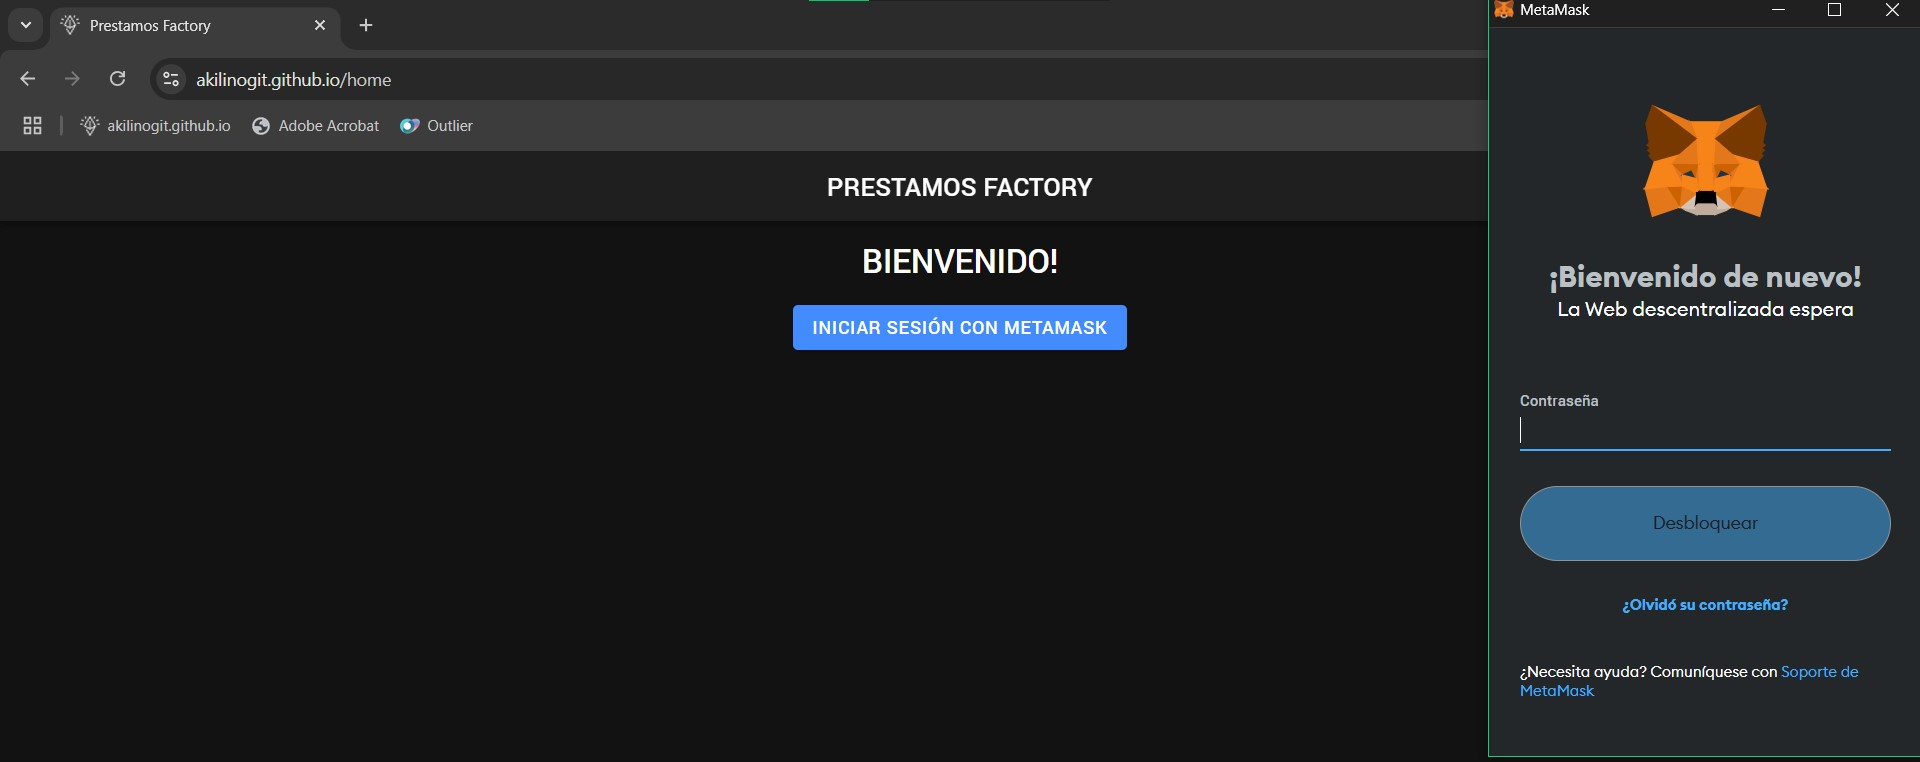
\includegraphics[width=\textwidth]{figures/resultados/metamask.jpg}
    \label{fig:metamask}
\end{figure}

    \item La utilización de \gls{metamask} no solo nos sirve para delegar 
    la identificación 
    sino también para delegar en una empresa externa la información que 
    identifica a 
    nuestros clientes, de forma que  no hace falta grabarla en la red.
    Esto nos ayuda con el \gls{os}~\ref{os:6} el cual busca este punto
    de unión. 
    Gracias a \gls{metamask} aunque existan cientos de operaciones económicas 
    reflejadas 
    en la red, sólo es posible comprobar la identidad de los participantes 
    de estas operaciones 
    a través de \gls{metamask} y las claves privadas de cada usuario.

    \item En el \gls{os}~\ref{os:2} se busca la eficiencia en la información y 
    las funciones del sistema para evitar el alto consumo de energía y \gls{gas} 
    a la hora 
    de ejecutar las transacciones en la red:

    Todas las funciones que tienen relación con la red son funciones muy atómicas 
    y sencillas evitando los grandes procesamientos de datos en la red aunque es 
    posible que la función que se encarga de comprobar los pagos de los contratos 
    de forma mensual pueda suponer una alta inversión por parte de la entidad
    financiera en caso de que tenga un volumen alto de préstamos, lo cual nos
    lleva a una posible actuación futura para limitar la cantidad de procesamiento 
    en esta acción.

    \item Haciendo referencia al \gls{os}~\ref{os:4} se adjuntan las siguientes
    imágenes del panel de control de la entidad prestamista en el que se muestran
    3 contratos de un usuario en curso antes y después de  la comprobación 
    mensual de los pagos de las cuotas.
    En ellas se pueden observar los distintos detalles:
    
    \begin{enumerate}
        \item El balance de la entidad después del pago de cuota del usuario
        aumenta correctamente
        \item Uno de los contratos no ha pagado correctamente la cuota 
        y se le ha aplicado automáticamente la penalización por impago.
        \item Uno de los contratos correctamente pagado ha reducido su deuda 
        restante y el número de cuotas restantes.
        \item En el caso del contrato que solo tenía una cuota restante, 
    ya no se muestra en la \gls{dapp} ya que no es necesario 
        replicar más esta información.
    \end{enumerate}
    Estas comprobaciones se pueden ver reflejadas con el cambio de información 
    correspondiente en la figura que muestra la información previa a la 
    comprobación mensual~\ref{fig:prechequeo} y tras la comprobación mensual 
    en la figura~\ref{fig:postchequeo}


\begin{figure}[H]
    \centering
    \caption{Información de contratos previa a la comprobación mensual en el recuadro amarillo y balance de la entidad prestamista en el recuadro blanco.}
    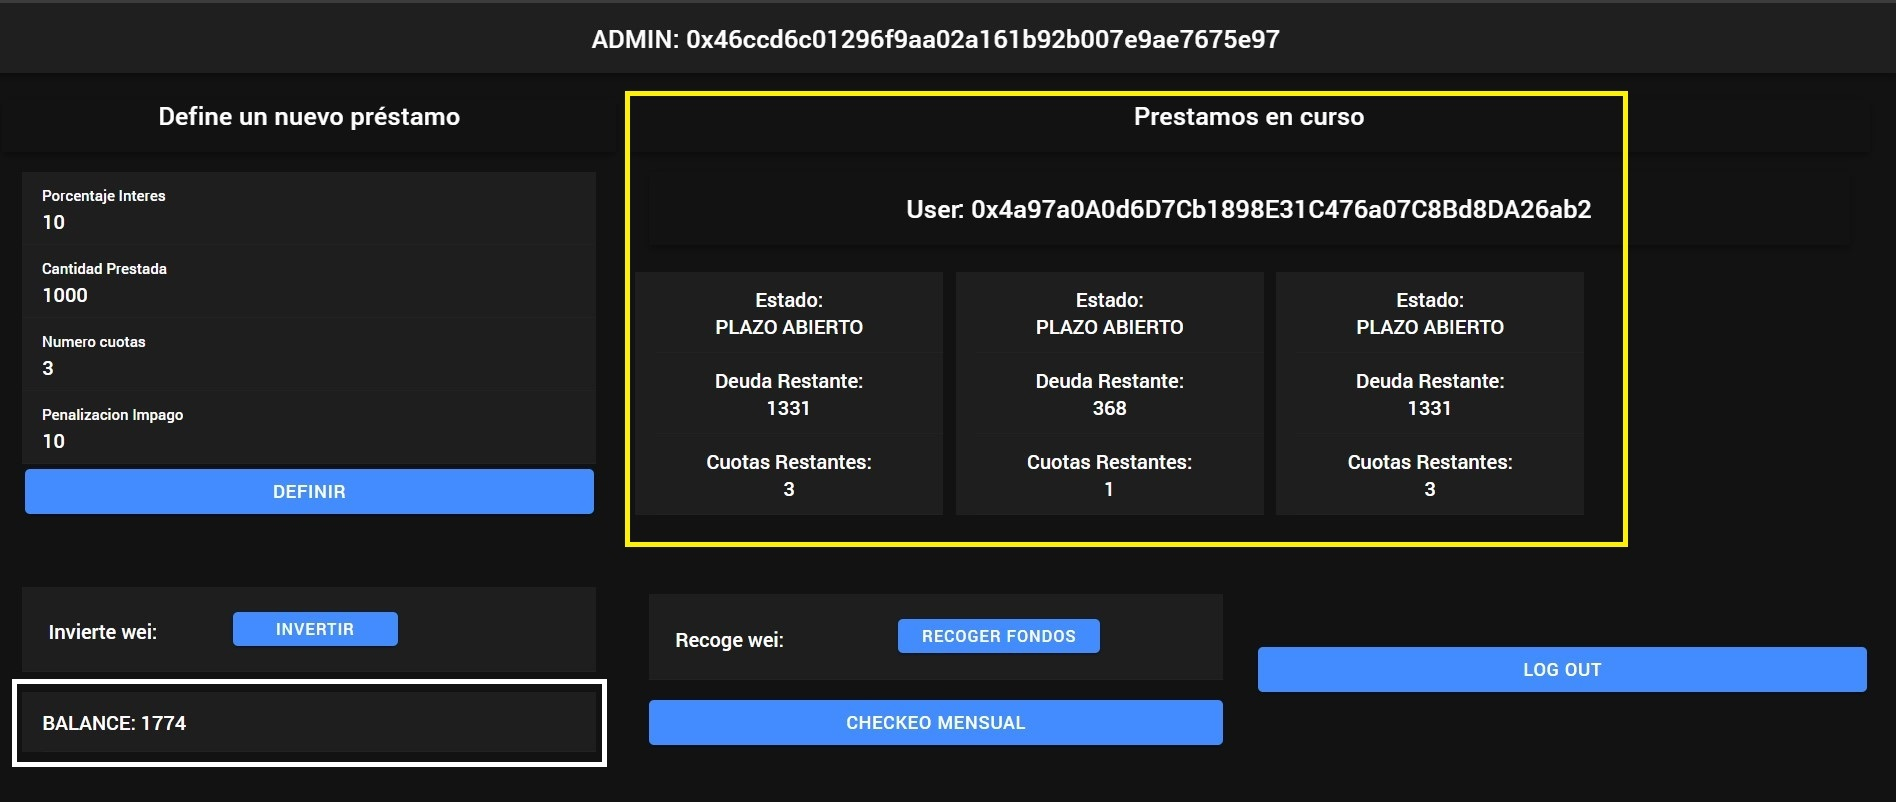
\includegraphics[width=\textwidth]{figures/resultados/prechequeo.jpg}
    \label{fig:prechequeo}
\end{figure}

\begin{figure}[H]
    \centering
    \caption{Información de contratos posterior a la comprobación mensual en el recuadro amarillo y balance de la entidad prestamista en el recuadro blanco.}
    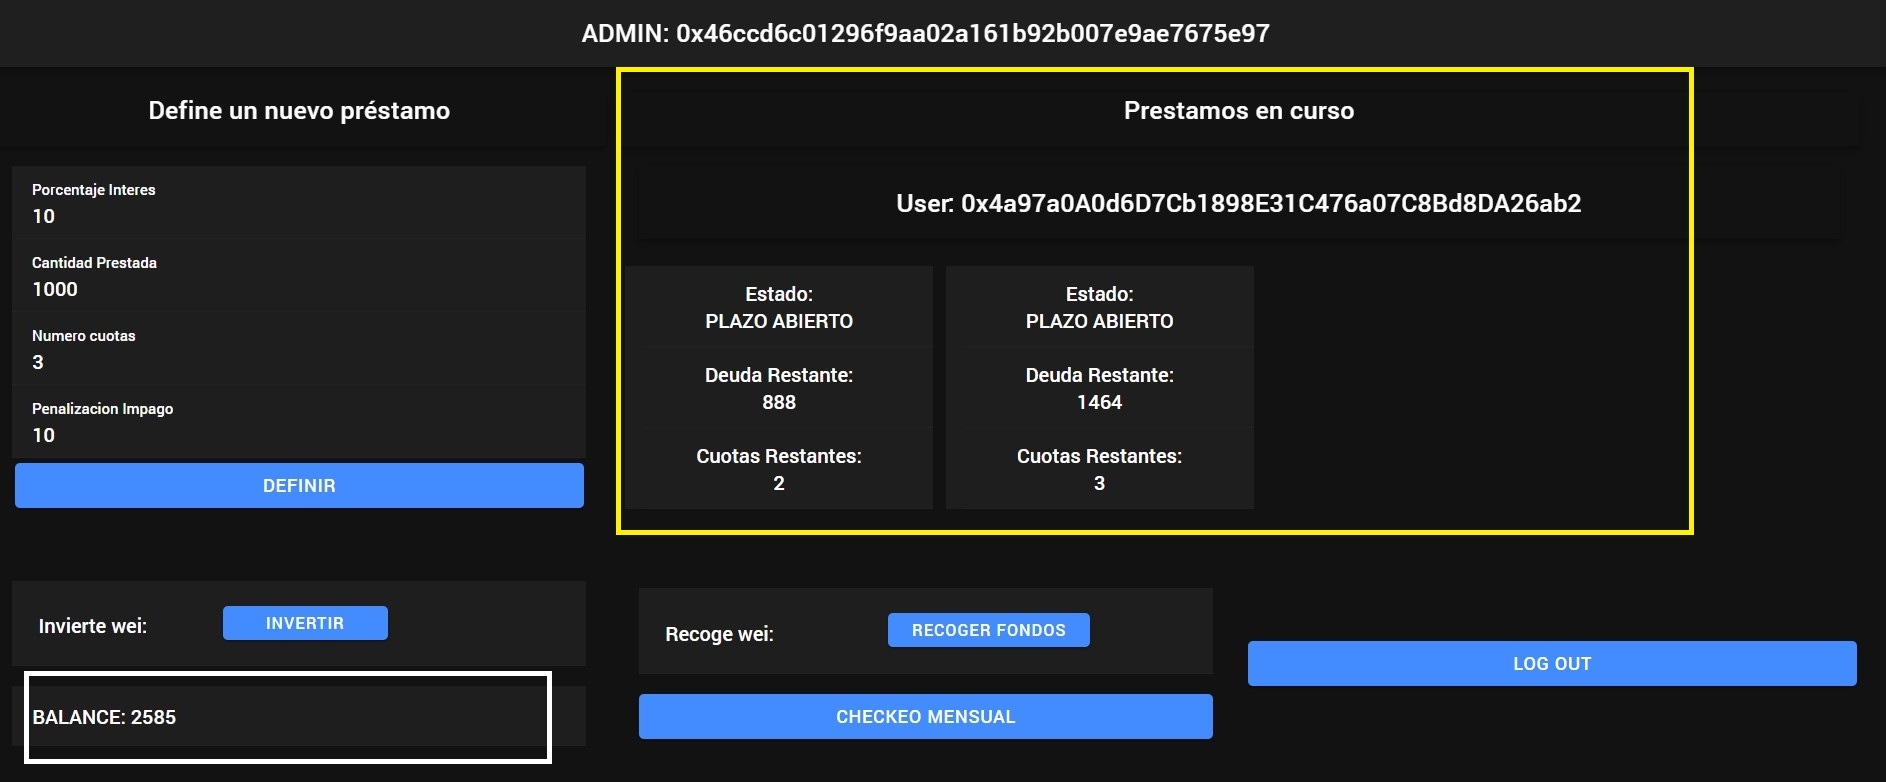
\includegraphics[width=\textwidth]{figures/resultados/postchequeo.jpg}
    \label{fig:postchequeo}
\end{figure}



Las últimas características declaradas junto con la posibilidad de que la 
organización del sistema pueda recibir los \gls{wei} del balance del sistema 
a través de la función \textit{Recoger Fondos} nos llevan al alcance del 
\gls{os}~\ref{os:7}, el cual busca encontrar la liquidez en este sistema.


\item En el \gls{os}~\ref{os:5} se contempla la posibilidad de personalizar 
los contratos accesibles para los distintos usuarios, esto se puede clasificar 
como inalcanzable para este proyecto debido a la necesidad de procesar
grandes cantidades de datos de clientes para poder crear un algoritmo y un 
sistema que cubra esta necesidad.

De momento existe la posibilidad de definir nuevos préstamos contratables en
el panel de control de la entidad prestamista.


\end{enumerate}

Para terminar de validar el \gls{op}~\ref{op:2} se adjunta captura de pantalla 
del panel de control del usuario en la figura~\ref{fig:paneluser} demostrando 
una interfaz unificada para el usuario.
        \begin{figure}[H]
    \centering
    \caption{Panel de control del usuario.}
    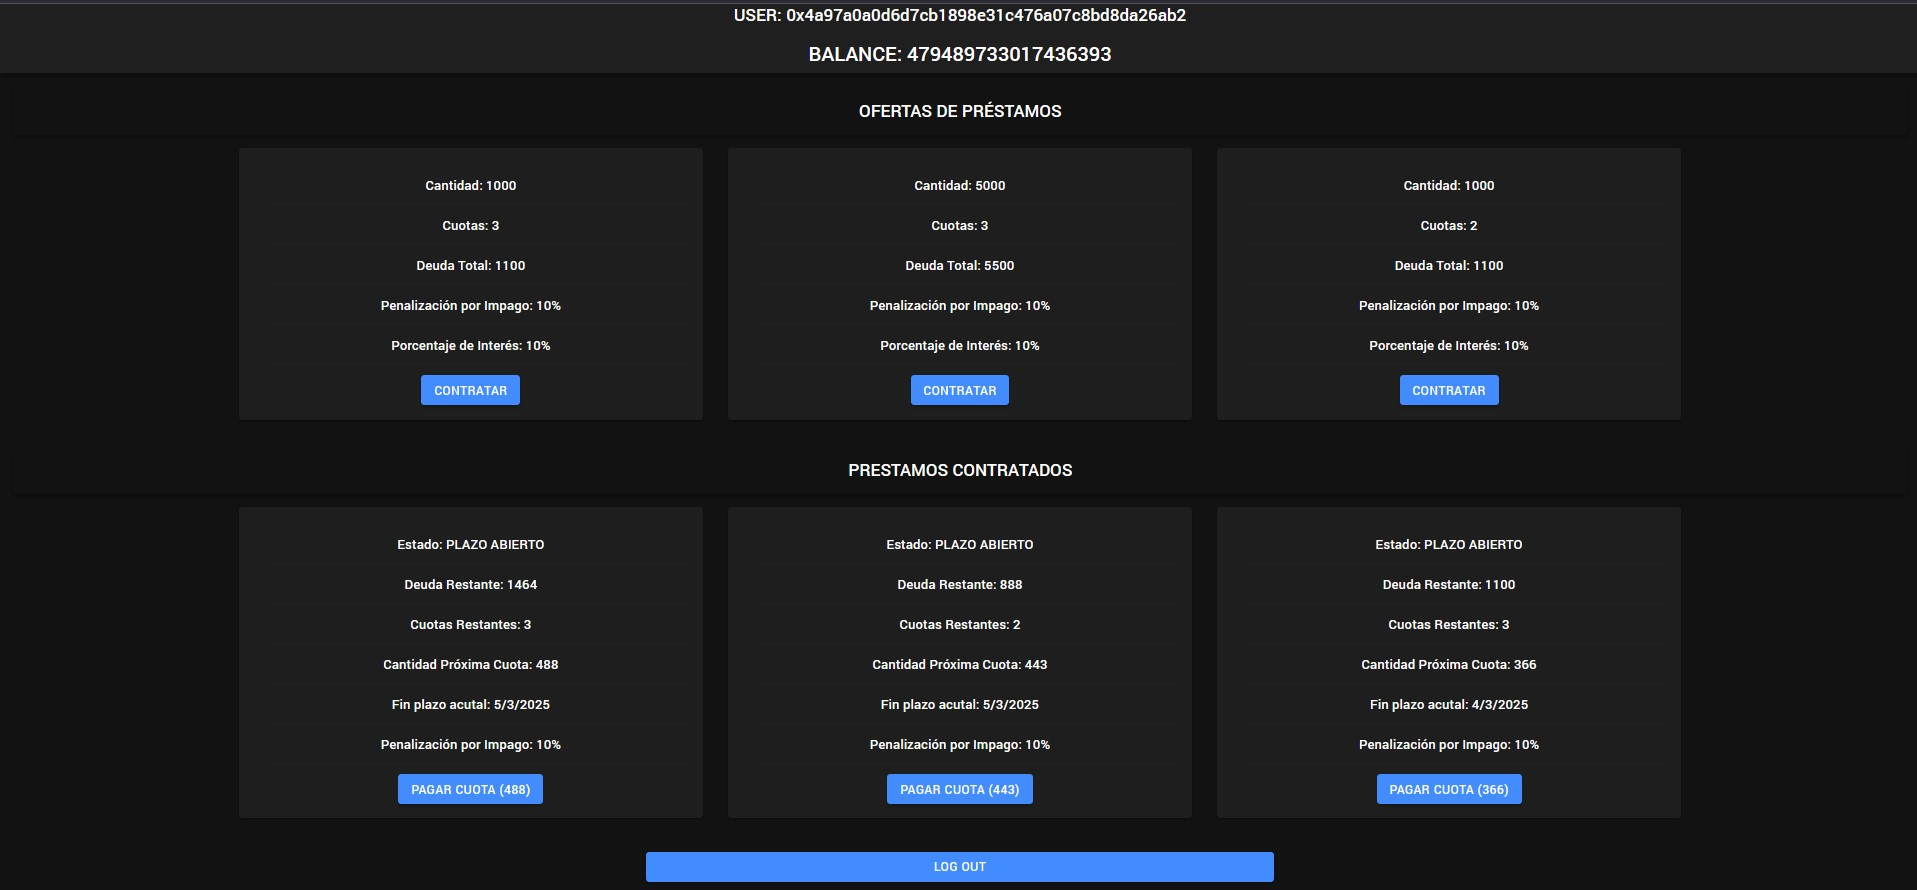
\includegraphics[width=\textwidth]{figures/resultados/paneluser.jpg}
    \label{fig:paneluser}
\end{figure}


Como última prueba de validación manual de este proyecto se realiza un ejemplo de 
contratación de préstamo adjuntando distintas capturas de la web
\href{https://sepolia.etherscan.io/}{Etherscan Sepolia} 
con las que se pueden comprobar distintos elementos relacionados con el proceso
que corroboran la veracidad del préstamo a través de la red 
\href{https://sepolia.dev/}{ Sepolia}.

\paragraph{Ejecución de préstamo de 1000~\gls{wei}}
\textbf{Contrato principal:} En la anterior figura~\ref{fig:postchequeo}
se puede comprobar que el balance del contrato principal es de 2585~\gls{wei}.

\textbf{Balance del usuario}: Después de la contratación del usuario,  
se puede ver a través de \href{https://sepolia.etherscan.io/}{Etherscan Sepolia}, 
tal y como se muestra en la figura~\ref{fig:Etherscan smart contract principal}, 
que:

    \begin{itemize}
        \item El balance del contrato ha disminuido 1000~\gls{wei}
        \item Se ha registrado una transacción de creación de contrato 
        (\textit{Contract Creation}), correspondiente al nuevo préstamo.
        \item Aunque debido al redondeo de la página aparezca otra transacción 
        de 0 \gls{eth}, viendo el balance se puede comprobar que es de 
        1000~\gls{wei} y han sido transferidos a la dirección del usuario.
    \end{itemize}

\begin{figure}[H]
    \centering
    \caption{Información de Etherscan del registro en la red SepoliaETH del 
    contrato inteligente principal}
    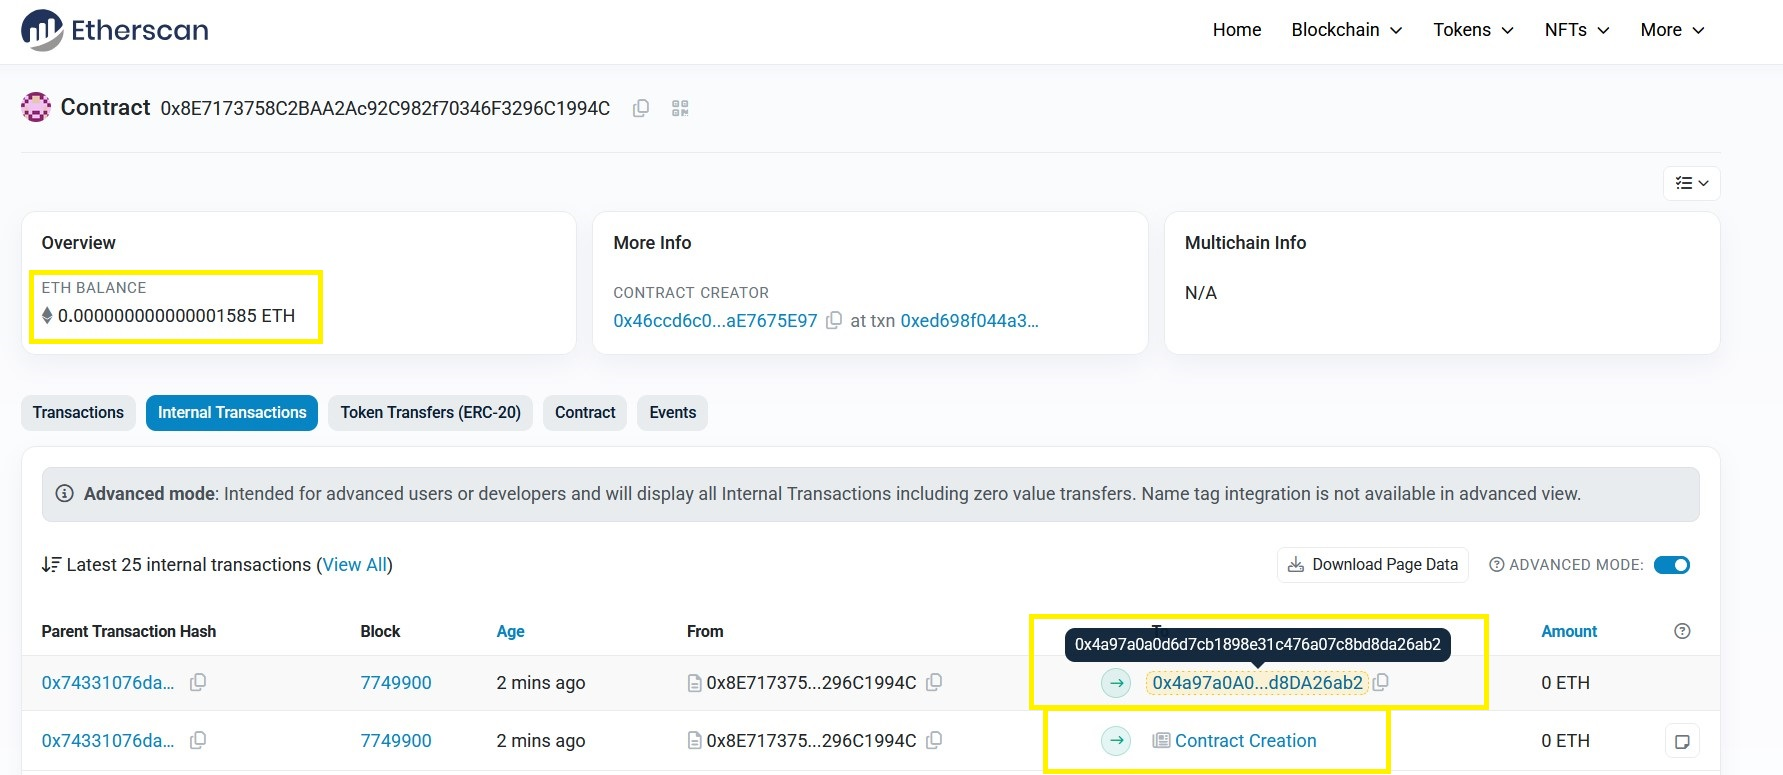
\includegraphics[width=\textwidth]{figures/resultados/createcontract.jpg}
    \label{fig:Etherscan smart contract principal}
\end{figure}

Se adjunta también otra captura de pantalla en la 
figura~\ref{fig:Etherscan comprobante de pago} de la información 
de la instancia generada del \gls{smartcontract} \textit{PrestamoCursando}

En la figura~\ref{fig:Etherscan comprobante de pago} también se puede observar
dentro del recuadro amarillo la primera transferencia recibida por parte del 
usuario con la cuota mensual. Esta cantidad de 366~\gls{wei} coincide correctamente
con el atributo \textit{Cantidad próxima cuota} del tercer préstamo contratado 
en el panel de usuario de la figura~\ref{fig:paneluser}.

Con esta comprobación de función de pago en 
\href{https://sepolia.etherscan.io/}{Etherscan Sepolia} 
se da por validado que todas las funciones del proyecto se reflejan en la red 
otorgando veracidad e inmutabilidad al proyecto.
\begin{figure}[H]
    \centering
    \caption{Registro en Sepolia en el que se puede ver una transacción o comprobante de pago Etherscan}
    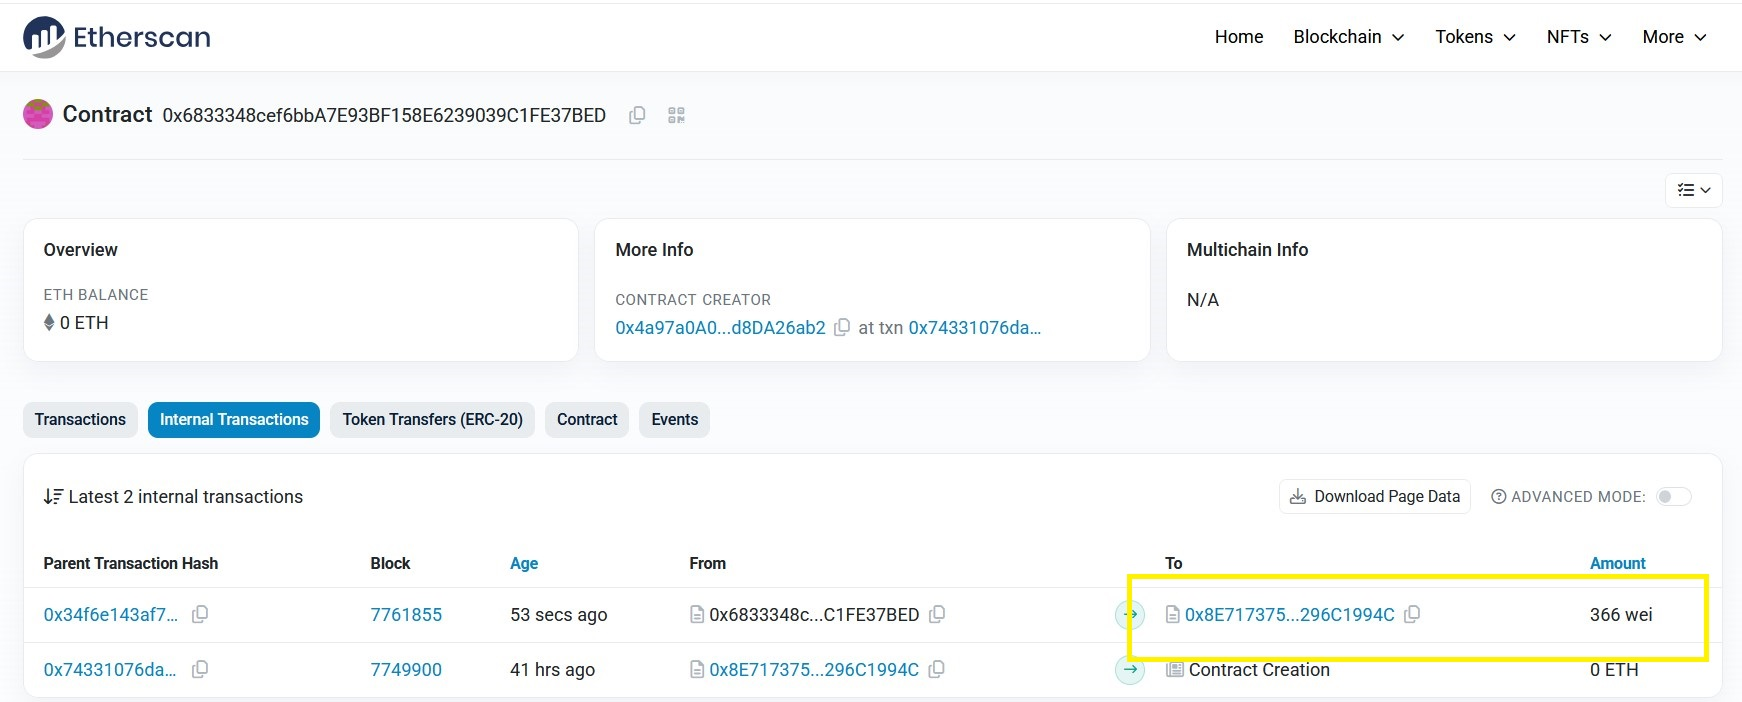
\includegraphics[width=\textwidth]{figures/resultados/pagoprestamo.jpg}
    \label{fig:Etherscan comprobante de pago}
\end{figure}


\subsection{Pruebas con Mocha}
Ya se ha visto el correcto funcionamiento de la aplicación a través de la
interfaz de usuario y la verificación de las transacciones en la red.
Pero para garantizar el correcto funcionamiento de los \glspl{smartcontract} en
situaciones distintas al correcto uso de la aplicación, 
se han desarrollado distintas pruebas unitarias utilizando la herramienta
\hyperref[sec:mochasection]{entorno de pruebas Mocha}.

Estas pruebas tienen como objetivo:
\begin{enumerate}
    \item Comprobar el funcionamiento de los contratos inteligentes.
    \item Verificar que las operaciones de préstamos funcionan correctamente.
    \item Detectar errores en condiciones normales y situaciones no permitidas.
    \item Comprobar las restricciones de acceso y los cambios de estado.
\end{enumerate}

\paragraph{Red de pruebas local:}
Para evitar utilizar una red pública se han desplegado los contratos sobre una red local utilizando la herramienta Ganache~\cite{[19]}.
Esto evita que aparezcan transacciones de prueba exponiendo información sensible del funcionamiento del  sistema en la red pública y 
permite la repetición de escenarios que son difíciles de reproducir en un entorno real, como que un usuario no pague su cuota mensual y se le aplique la penalización correspondiente.
\paragraph{Cuentas utilizadas para las pruebas:}
La herramienta de creación de red local virtual es la encargada de generar distintas cuentas con las que interactuar en la red.
Se han utilizado 3 cuentas para realizar las pruebas unitarias:
\begin{enumerate}
    \item Una cuenta propietaria del sistema
    \item Dos cuentas de usuario que solicitan el préstamo
\end{enumerate}
\paragraph{Contratos inteligentes puestos a prueba:}
Las pruebas se han hecho sobre el motor de este sistema, es decir, sobre los
\glspl{smartcontract} que definen el funcionamiento del sistema de préstamos.
Estos contratos se pueden ver en el anexo ~\ref{anexo:smartcontracts} y son los 
ya comentados \textit{PrestamosFactory} y \textit{PrestamoCursando}.

\paragraph{Tecnología de las pruebas:}
Las pruebas se han desarrollado utilizando JavaScript, el entorno de pruebas Mocha y
el módulo \texttt{assert} de Node.js para las aserciones.
Estas pruebas se pueden encontrar en el anexo~\ref{anexo:mochatest}.

\paragraph{Desarrollo de las pruebas: Variables previas y condiciones iniciales:}
Previo al desarrollo puro de las pruebas, antes de cada ejecución se deben dar las condiciones iniciales para que las pruebas puedan ejecutarse correctamente.
El proceso de preparación de las pruebas consiste en desplegar los contratos en la red local y establecer las condiciones iniciales para cada prueba.
Para ello se han realizado los siguientes pasos:
\begin{enumerate}
    \item \textbf{Compilación en local de los contratos inteligentes:} A través de la
    herramienta \textit{Truffle} se compilan los \glspl{smartcontract} 
    previamente para que la red sea capaz de entender sus funciones.
    Esta compilación genera un archivo .json con las funciones del \gls{smartcontract} 
    parametrizadas para que la red sea capaz de interactuar con él.
    \item \textbf{Obtención de cuentas:} Se obtienen las cuentas necesarias para realizar las pruebas.
    \item \textbf{Despliegue del contrato en la red:} En el desarrollo de las pruebas se hace uso del archivo .json de la compilación y se despliega el contrato a testear en la red local de pruebas.
            \begin{lstlisting}[language=Solidity, caption={Despliegue de contrato en la red local}]
                    describe('Prestamos factory test', () => {

                    before( async() => {  
                        accounts = await web3.eth.getAccounts();
                        factory = await new web3.eth.Contract(prestamosFactoryBuild.abi)
                            .deploy({data: prestamosFactoryBuild.evm.bytecode.object})
                            .send({ from: accounts[0], gas: 6721975});
                        
                        console.log('contract address:'+ factory.options.address);
                        console.log('Owner: ' + accounts[0]);
                        
                        
                    } );

                \end{lstlisting}

    \item \textbf{Establecimiento del estado inicial:} En el caso de las pruebas para
    los \textit{PrestamoCursando}, se establecen primero las variables previas
    necesarias para la contratación de un préstamo.
    Estas son:
    \begin{enumerate}
        \item \textbf{Introducción de fondos:} El sistema de préstamos necesita
        fondos previos para que se le puedan solicitar préstamos.
        \item \textbf{Creación de un tipo de préstamo:} Se crea un tipo de
        préstamo con las características necesarias para la prueba.
        \item \textbf{Creación de contratos de préstamo y obtención de sus
        direcciones:} De esta manera se obtiene la forma de acceder a los
        contratos sobre los que se ejecutarán las pruebas.
    \end{enumerate}
    
\begin{lstlisting}[language=Solidity, caption={Parametrización de préstamos en curso}]
    describe('Prestamos Cursando test', async () => {
    //INICIALIZAR PRESTAMOS EN CURSO
    before(async() => {  
        //Inicializar cuentas
        accounts = await web3.eth.getAccounts();
        
        
        //Inicializar contract factory
        factory = await new web3.eth.Contract(prestamosFactoryBuild.abi)
            .deploy({data: prestamosFactoryBuild.evm.bytecode.object})
            .send({ from: accounts[0], gas: 6721975});
            

        //Invertir para poder crear nuevos contratos
        await factory.methods.invertir().send({
                from: accounts[0],
                value: web3.utils.toHex(10000)
            });
        //Definir préstamo
        await factory.methods.definirPrestamo(10,1000,2,10).send({from: accounts[0],
            gas: web3.utils.toHex(2000000)});
        //Contratar préstamos
        await factory.methods.contratarPrestamo(accounts[1],0).send({from: accounts[1],
            gas: web3.utils.toHex(2000000)});
        await factory.methods.contratarPrestamo(accounts[2],0).send({from: accounts[2],
            gas: web3.utils.toHex(2000000)});

        [prestamo1address]=await factory.methods.verContratos(accounts[1]).call({from: accounts[1]});
        [prestamo2address]=await factory.methods.verContratos(accounts[2]).call({from: accounts[2]});
        
        prestamo1 = await new web3.eth.Contract(prestamoCursandoBuild.abi,prestamo1address);
        prestamo2 = await new web3.eth.Contract(prestamoCursandoBuild.abi,prestamo2address);
        
    });
    \end{lstlisting}

    \item \textbf{Descripción de las pruebas:} El contenido de las pruebas se puede ver en
    los dos ficheros del anexo ~\ref{anexo:mochatest} y se describen a 
    continuación:
            \begin{enumerate}
                \item \textbf{Pruebas del \texttt{PrestamosFactory}}

                En \path{test_prestamos_factory.js} se comprueba principalmente el \textbf{funcionamiento de PrestamosFactory y sus restricciones}:

                \begin{enumerate}
                    \item \textbf{Despliegue del contrato}: se verifica que el \texttt{PrestamosFactory} se despliega correctamente y obtiene una dirección.
                    \item \textbf{Control de acceso}: se comprueba que determinadas funciones únicamente pueden ser ejecutadas por el \texttt{owner}.
                    \item \textbf{Ingreso de fondos}: se comprueba que \texttt{invertir()} incrementa correctamente el saldo del Factory.
                    \item \textbf{Consulta de saldo}: se verifica que \texttt{getBalance()} devuelve el saldo real del contrato.
                    \item \textbf{Estado inicial}: se comprueba que inicialmente no existen clientes, tipos de préstamo ni préstamos en curso.
                    \item \textbf{Retirada de fondos}: se verifica que \texttt{recolectarFondos()} reduce correctamente el saldo del Factory.
                    \item \textbf{Validación de parámetros}: se prueban valores incorrectos para los porcentajes de intereses y penalizaciones, comprobando que las operaciones son rechazadas.
                    \item \textbf{Creación de tipos de préstamo}: se comprueba que \texttt{definir\allowbreak{}Prestamo()} crea correctamente un nuevo producto y genera el evento correspondiente.
                    \item \textbf{Consulta de tipos de préstamo}: se verifica que los datos almacenados coinciden con los valores introducidos.
                    \item \textbf{Contratación de préstamos}: se comprueba tanto la contratación correcta como situaciones en las que la operación debe fallar.
                    \item \textbf{Consulta de préstamos de un usuario}: se verifica que \texttt{ver\allowbreak{}Contratos()} devuelve los contratos correspondientes.
                    \item \textbf{Intento de eliminar un préstamo no finalizado}: se comprueba que esta operación no está permitida.
                \end{enumerate}

                \item \textbf{Pruebas del \texttt{PrestamoCursando}}

                El segundo archivo prueba el \textbf{ciclo de vida de un préstamo individual}.

                Se parte de una situación preparada con:

                \begin{enumerate}
                    \item Factory desplegado.
                    \item Fondos introducidos.
                    \item Tipo de préstamo creado.
                    \item Dos préstamos contratados por usuarios diferentes.
                \end{enumerate}

                A partir de ahí se prueban:

                \begin{enumerate}
                    \item \textbf{Control de acceso a la información}: un usuario diferente al prestatario no puede consultar la información privada del préstamo.
                    \item \textbf{Consulta de información del préstamo}: se comprueban importe prestado, deuda, cuota mensual, número de cuotas, estado, prestatario, etc.
                    \item \textbf{Restricción temporal}: se comprueba que no se puede realizar el chequeo mensual antes de que haya transcurrido el tiempo establecido.
                    \item \textbf{Pago de una cuota}: se realiza un pago y se comprueba que:
                    \begin{enumerate}
                        \item[a)] disminuye el número de cuotas restantes;
                        \item[b)] disminuye la deuda;
                        \item[c)] cambia el estado del préstamo.
                    \end{enumerate}
                    \item \textbf{Transferencia de fondos}: se verifica que el dinero pagado vuelve correctamente al \texttt{PrestamosFactory} y que su balance es el esperado.
                    \item \textbf{Chequeo mensual}: se simula el paso del tiempo y se comprueba que el chequeo:
                    \begin{enumerate}
                        \item[a)] actualiza el estado del préstamo;
                        \item[b)] aplica una penalización al préstamo que no ha sido pagado.
                    \end{enumerate}
                    \item \textbf{Finalización del préstamo}: se paga la última cuota y se comprueba que el préstamo pasa al estado de finalizado.
                    \item \textbf{Eliminación de préstamos finalizados}: después del chequeo mensual se comprueba que el contrato finalizado deja de aparecer entre los préstamos activos del usuario y que se actualiza la lista de clientes.
                \end{enumerate}
            \end{enumerate}

    \item \textbf{Comprobación de las pruebas} Tras la ejecución de las pruebas, se comprueba que los resultados obtenidos son los esperados y que el sistema funciona correctamente.
     Para ello se utilizan las funciones de aserción de Node.js, que permiten comparar los resultados obtenidos con los esperados y generar un informe de las pruebas realizadas.
       \end{enumerate}
    
\paragraph{Resultados} Tras el desarrollo y ejecución de las pruebas se puede comprobar que el sistema funciona correctamente y que se cumplen los objetivos planteados.
    A su vez se han encontrado 2 situaciones que no se contemplaban en el diseño inicial.
\begin{enumerate}
    \item La función \texttt{setIndex} actualiza el índice de un préstamo.
    En el código del anexo está restringida mediante \texttt{onlyContractFactory},
    que comprueba que el emisor sea el contrato principal y tuviese
        el archivo compilado del contrato podría acceder directamente a esta 
        función y simular que es uno de los contratos en curso 
        y modificar el índice de los contratos de un usuario pudiendo quedar 
        invisibles.
        \item La función que comprueba mensualmente el estado de todos los 
        contratos del sistema se demora más segundos de los que el tiempo de espera de Mocha tiene por defecto por lo que se ha tenido que aumentar.
\end{enumerate}

\subsection{Validación del proyecto después de pruebas}
Durante la ejecución de las pruebas de este proyecto y la simulación de un entorno real se ha visto que un sistema como este puede llegar a niveles de producción
en un entorno real. Dejando aparte la necesidad de un desarrollo futuro para
añadir actores y elementos necesarios para un sistema de préstamos real
a nivel técnico se afirma que la tecnología es viable.

\subsection{Viabilidad económica}
Tras estudiar los gastos de \gls{gas} en los registros de 
\href{https://sepolia.etherscan.io/}{Etherscan Sepolia} se puede comprobar 
que los gastos de contratar un préstamo
dependen mucho del precio del \gls{gas} en el momento de contratación, 
el cual varía de forma muy dinámica dependiendo de la congestión de la red.
En el proceso de validación se han ejecutado
 transferencias de préstamo con costes desde 0,46 dólares hasta 30,49 dólares.
 Esto puede crear un cuello de botella de entrada de préstamos en caso de que 
 se dependa en exceso de esta variable obligando 
a la gestión del sistema a retrasar contratos y operaciones cuando el coste 
sea muy alto o directamente pasar los costes a los clientes.
Por otro lado, independientemente de esta variable, a nivel técnico se ha 
comprobado que en el momento en el que se comprueba si todos los préstamos
 han sido pagados o no
la cantidad de procesamiento aumenta linealmente por el número de contratos 
en el sistema, sumando esto a un alto coste del gas se podría crear un bloqueo
total del sistema,
por lo que sería obligatorio optimizar la forma en la que se realiza este 
chequeo.


